\section{The case $[5, 7]_3$}
\begin{theorem}
    Let $p = (p_3, p_4, p_5, \dots, p_n)$ be a given sequence satisfying equation \ref{eq_valence_3}, then there exists $r \in \nats$ for which $p + r [5, 7]_3$ is $3$-realizable.
    \begin{proof}
      \heartpar{
  The proof starts by using the construction given by Eberhards Theorem \ref{thm_eberhard}(\ref{thm_eberhard_3}). This results in a realization of $p$ which has many more hexagons then needed. The next step is to remove these hexagons and replace them by pentagons and heptagons. To further proceed, one adds a ring of hexagons around each polygon in the realization, these will be replaced immediately but serve the purpose of adding space around each polygon which can be used for replacement with pentagons and heptagons. The process is illustrated below:
}
  \begin{figure}[htpp]
    \centering
    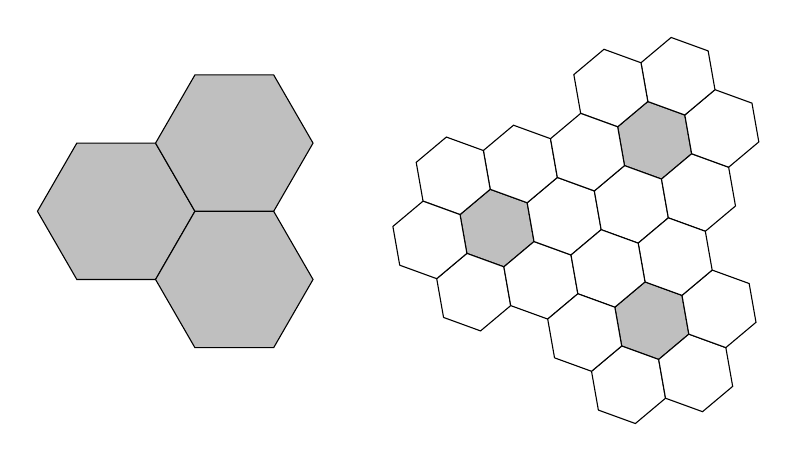
\begin{tikzpicture}
      \matrix (m) [ column sep=1cm] {
          \begin{scope}[xscale=1.0, yscale=0.866]
            \filldraw[fill=gray!50!white] (0, 1) -- ++(0.5, -1) -- ++(1, 0) -- ++(0.5, 1) -- ++(-0.5, 1) -- ++(-1, 0) -- ++(-0.5, -1);
            \filldraw[fill=gray!50!white] (1.5, 0) -- ++(0.5, -1) -- ++(1, 0) -- ++(0.5, 1) -- ++(-0.5, 1) -- ++(-1, 0) -- ++(-0.5, -1);
            \filldraw[fill=gray!50!white] (1.5, 2) -- ++(0.5, -1) -- ++(1, 0) -- ++(0.5, 1) -- ++(-0.5, 1) -- ++(-1, 0) -- ++(-0.5, -1);
          \end{scope}
        &


          \begin{scope}[rotate=40, xscale=1.0, yscale=0.866, scale=0.5] 
            \filldraw[fill=gray!50!white] (0, 1) -- ++(0.5, -1) -- ++(1, 0) -- ++(0.5, 1) -- ++(-0.5, 1) -- ++(-1, 0) -- ++(-0.5, -1);
            \filldraw[fill=white] (-1.5, 0) -- ++(0.5, -1) -- ++(1, 0) -- ++(0.5, 1) -- ++(-0.5, 1) -- ++(-1, 0) -- ++(-0.5, -1);
          \filldraw[fill=white] (0, -1) -- ++(0.5, -1) -- ++(1, 0) -- ++(0.5, 1) -- ++(-0.5, 1) -- ++(-1, 0) -- ++(-0.5, -1);
          \filldraw[fill=white] (1.5, 0) -- ++(0.5, -1) -- ++(1, 0) -- ++(0.5, 1) -- ++(-0.5, 1) -- ++(-1, 0) -- ++(-0.5, -1);
          \filldraw[fill=white] (1.5, 2) -- ++(0.5, -1) -- ++(1, 0) -- ++(0.5, 1) -- ++(-0.5, 1) -- ++(-1, 0) -- ++(-0.5, -1);
          \filldraw[fill=white] (0, 3) -- ++(0.5, -1) -- ++(1, 0) -- ++(0.5, 1) -- ++(-0.5, 1) -- ++(-1, 0) -- ++(-0.5, -1);
          \filldraw[fill=white] (-1.5, 2) -- ++(0.5, -1) -- ++(1, 0) -- ++(0.5, 1) -- ++(-0.5, 1) -- ++(-1, 0) -- ++(-0.5, -1);

          \filldraw[fill=gray!50!white] (4.5, 0) -- ++(0.5, -1) -- ++(1, 0) -- ++(0.5, 1) -- ++(-0.5, 1) -- ++(-1, 0) -- ++(-0.5, -1);
          \filldraw[fill=white] (3, -1) -- ++(0.5, -1) -- ++(1, 0) -- ++(0.5, 1) -- ++(-0.5, 1) -- ++(-1, 0) -- ++(-0.5, -1);
          \filldraw[fill=white] (4.5, -2) -- ++(0.5, -1) -- ++(1, 0) -- ++(0.5, 1) -- ++(-0.5, 1) -- ++(-1, 0) -- ++(-0.5, -1);
          \filldraw[fill=white] (6, -1) -- ++(0.5, -1) -- ++(1, 0) -- ++(0.5, 1) -- ++(-0.5, 1) -- ++(-1, 0) -- ++(-0.5, -1);
          \filldraw[fill=white] (6, 1) -- ++(0.5, -1) -- ++(1, 0) -- ++(0.5, 1) -- ++(-0.5, 1) -- ++(-1, 0) -- ++(-0.5, -1);
          \filldraw[fill=white] (4.5, 2) -- ++(0.5, -1) -- ++(1, 0) -- ++(0.5, 1) -- ++(-0.5, 1) -- ++(-1, 0) -- ++(-0.5, -1);
          \filldraw[fill=white] (3, 1) -- ++(0.5, -1) -- ++(1, 0) -- ++(0.5, 1) -- ++(-0.5, 1) -- ++(-1, 0) -- ++(-0.5, -1);
          
          \filldraw[fill=gray!50!white] (1.5, -4) -- ++(0.5, -1) -- ++(1, 0) -- ++(0.5, 1) -- ++(-0.5, 1) -- ++(-1, 0) -- ++(-0.5, -1);
          \filldraw[fill=white] (0, -5) -- ++(0.5, -1) -- ++(1, 0) -- ++(0.5, 1) -- ++(-0.5, 1) -- ++(-1, 0) -- ++(-0.5, -1);
          \filldraw[fill=white] (1.5, -6) -- ++(0.5, -1) -- ++(1, 0) -- ++(0.5, 1) -- ++(-0.5, 1) -- ++(-1, 0) -- ++(-0.5, -1);
          \filldraw[fill=white] (3, -5) -- ++(0.5, -1) -- ++(1, 0) -- ++(0.5, 1) -- ++(-0.5, 1) -- ++(-1, 0) -- ++(-0.5, -1);
          \filldraw[fill=white] (3, -3) -- ++(0.5, -1) -- ++(1, 0) -- ++(0.5, 1) -- ++(-0.5, 1) -- ++(-1, 0) -- ++(-0.5, -1);
          \filldraw[fill=white] (1.5, -2) -- ++(0.5, -1) -- ++(1, 0) -- ++(0.5, 1) -- ++(-0.5, 1) -- ++(-1, 0) -- ++(-0.5, -1);
          \filldraw[fill=white] (0, -3) -- ++(0.5, -1) -- ++(1, 0) -- ++(0.5, 1) -- ++(-0.5, 1) -- ++(-1, 0) -- ++(-0.5, -1);
        \end{scope};
        \\
      };
  \end{tikzpicture}
  \end{figure}


  One now chooses a set $S$ of hexagons one wants to keep, $|S| = p_6$. Each hexagon not in $S$ and the surrounding six hexagons are replaced by the following structure: 

  \begin{figure}[htpp]
    \centering
    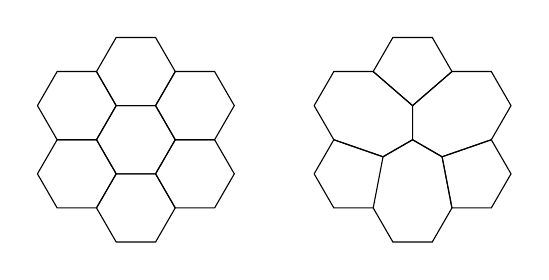
\begin{tikzpicture}
      \matrix (m) [ column sep=1cm] {
        \begin{scope}[xscale=1.0, yscale=0.866, scale=0.5]
          \draw (0, 1) -- ++(0.5, -1) -- ++(1, 0) -- ++(0.5, 1) -- ++(-0.5, 1) -- ++(-1, 0) -- ++(-0.5, -1);
          \draw (-1.5, 0) -- ++(0.5, -1) -- ++(1, 0) -- ++(0.5, 1) -- ++(-0.5, 1) -- ++(-1, 0) -- ++(-0.5, -1);
          \draw (0, -1) -- ++(0.5, -1) -- ++(1, 0) -- ++(0.5, 1) -- ++(-0.5, 1) -- ++(-1, 0) -- ++(-0.5, -1);
          \draw (1.5, 0) -- ++(0.5, -1) -- ++(1, 0) -- ++(0.5, 1) -- ++(-0.5, 1) -- ++(-1, 0) -- ++(-0.5, -1);
          \draw (1.5, 2) -- ++(0.5, -1) -- ++(1, 0) -- ++(0.5, 1) -- ++(-0.5, 1) -- ++(-1, 0) -- ++(-0.5, -1);
          \draw (0, 3) -- ++(0.5, -1) -- ++(1, 0) -- ++(0.5, 1) -- ++(-0.5, 1) -- ++(-1, 0) -- ++(-0.5, -1);
          \draw (-1.5, 2) -- ++(0.5, -1) -- ++(1, 0) -- ++(0.5, 1) -- ++(-0.5, 1) -- ++(-1, 0) -- ++(-0.5, -1);
        \end{scope};

        &

        \begin{scope}[xscale=1.0, yscale=0.866, scale=0.5] 
          \draw (-1.5, 0) -- ++(0.5, -1) -- ++(1, 0) -- ++(0.25, 1.5) -- ++(-1.25, 0.5) -- ++(-0.5, -1);
          \draw (0, -1) -- ++(0.5, -1) -- ++(1, 0) -- ++(0.5, 1) -- ++(-0.25, 1.5) -- ++(-0.75, 0.5) -- ++(-0.75, -0.5);
          \draw (1.75, 0.5) -- ++(0.25, -1.5) -- ++(1, 0) -- ++(0.5, 1) -- ++(-0.5, 1) -- ++(-1.25, -0.5);
          \draw (1, 1) -- ++(0.75, -0.5) -- ++(1.25, 0.5) -- ++(0.5, 1) -- ++(-0.5, 1) -- ++(-1, 0) -- ++(-1, -1);
          \draw (0, 3) -- ++(1, -1) -- ++(1, 1) -- ++(-0.5, 1) -- ++(-1, 0) -- ++(-0.5, -1);
          \draw (-1.5, 2) -- ++(0.5, -1) -- ++(1.25, -0.5) -- ++(0.75, 0.5) -- ++(0, 1) -- ++(-1, 1) -- ++(-1, 0) -- ++(-0.5, -1);
        \end{scope};
        
        \\
      };
  \end{tikzpicture}
  \end{figure}

  For the remaining hexagons and all other kinds of polygons this ring structure is replaced differently, for each $n$-gon $n$ pentagons and $n$ heptagons replace the ring of hexagons:


    \begin{figure}[htpp]
    \centering
    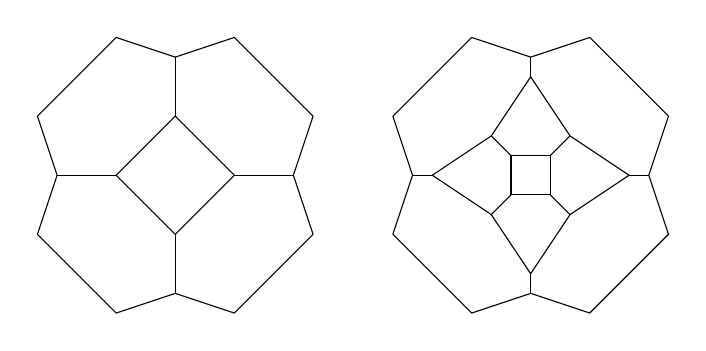
\begin{tikzpicture}
      \matrix (m) [ column sep=1cm] {

        \begin{scope}[scale=0.25] 
          \draw (-3, 0) -- (0, -3) -- (3, 0) -- (0, 3) -- (-3, 0);
          \draw (-3, 0) -- (-6, 0);
          \draw (0, -3) -- (0, -6);
          \draw (3, 0) -- (6, 0);
          \draw (0, 3) -- (0, 6);
          \draw (-6, 0) -- (-7, -3) -- (-3, -7) -- (0, -6) -- (3, -7) -- (7, -3) -- (6, 0) -- (7, 3) -- (3, 7) -- (0, 6) -- (-3, 7) -- (-7, 3) -- (-6, 0);
        \end{scope}
        &
        \begin{scope}[scale=0.25] 
          \draw (-6, 0) -- (-7, -3) -- (-3, -7) -- (0, -6) -- (3, -7) -- (7, -3) -- (6, 0) -- (7, 3) -- (3, 7) -- (0, 6) -- (-3, 7) -- (-7, 3) -- (-6, 0);
          \draw (-5, 0) -- (-6, 0);
          \draw (0, -5) -- (0, -6);
          \draw (5, 0) -- (6, 0);
          \draw (0, 5) -- (0, 6);

          \draw (-5, 0) -- (-2, -2) -- (0, -5) -- (2, -2) -- (5, 0) -- (2, 2) -- (0, 5) -- (-2, 2) -- (-5, 0);
          \draw (-2, -2) -- (-1, -1);
          \draw (2, -2) -- (1, -1);
          \draw (2, 2) -- (1, 1);
          \draw (-2, 2) -- (-1, 1);
          
          \draw (-1, -1) -- (1, -1) -- (1, 1) -- (-1, 1) -- (-1, -1);

        \end{scope}
        
        \\
      };
  \end{tikzpicture}
  \end{figure}
  This finishes the proof.
\end{proof}
\end{theorem}


